\chapter{Ergebnisse}   \label{ch_4}
Im folgenden Kapitel werden die durchgeführten statistischen Berechnungen dargestellt. Zu Beginn werden die deskriptiven Ergebnisse beschrieben und mit den Normwerten verglichen, woraufhin die statistische Überprüfung der Manipulation folgt. Im inferenzstatistischen Unterkapitel wird mit der Prüfung der Vorraussetzung der einzelnen Test mathematisch dargestellt und abschließend werden die Ergebnisse der drei Hypothesen präsentiert. Die ausführliche Interpretation der Ergebnisse geschieht im nachkommenden Kapitel ~\ref{ch_5}.

\section{Deskriptive Ergebnisse}    \label{sec_4.1}
Die Fallvignetten wießen, bei einem $Min$~=~1 und einem $Max$~=~101, einen Mittelwert von $M$~=~26.46 ($SD$~=~27.98) auf. Der Median lag bei $Mdn$~=~19. Die am häufigsten verteilten Werte liegen an den beiden Extremen bei 1.00 und 101.00 und bilden eine bimodale Verteilung. Bei einer Schiefe von 1.17 und Kurtosis von 0.53, liegt eine rechstschiefe bzw. linkssteile und steilgipflige Verteilung vor. Abbildung~\ref{Histogramm VicBlame} stellt die unimodale Verteilung der Verantwortungszuschreibung bildlich da. Die vorhandenen Ausreißer befinden sich alle unter der Ausscheidungsgrenze.
% Modus: 1.00 und 101.00
\begin{figure}[htb]
    \centering
        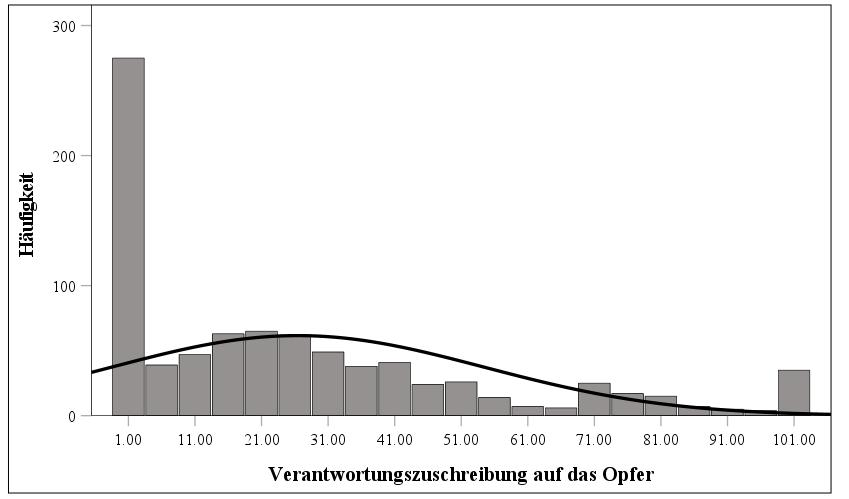
\includegraphics[width=0.8\linewidth]{Histogramm VicBlame.jpg}
        \caption[Histogramm Verantwortungszuschreibung]{Verteilung der Verantwortungszuschreibung.}
        \label{Histogramm VicBlame}
\end{figure}



Der DVMAS zeigte einen Mittelwert von $M$~=~2.60 ($SD$~=~0.80) und einen Median von $Mdn$~=~2.5. Der geringste Wert war dabei $Min$~=~1 und der höchsete $Max$~=~5.56. Die häufigsten Werte lagen bei 2.11 und 2.67 und bilden eine bimodale Verteilung. Eine Schiefe von 0.60 bildet eine leicht rechstschiefe Verteilung. Die Kurtosis von 0.09 bildet eine leicht steilere Verteilung, als die Normalverteilung. Beide Werte weichen demzufolge leicht von einer Normalverteilung ab ($M$~=~2.30, $SD$~=~0.85 und Schiefe~=~0.63). 
Die Abbildung~\ref{Histogramm DVMAS} bildet die beschriebenen Werte dieser Studie bildlich ab. Die vorhandenen Ausreißer befinden sich alle unter der Ausscheidungsgrenze.
% Modus: 2.11, 2.67
\begin{figure}[htb]
    \centering
        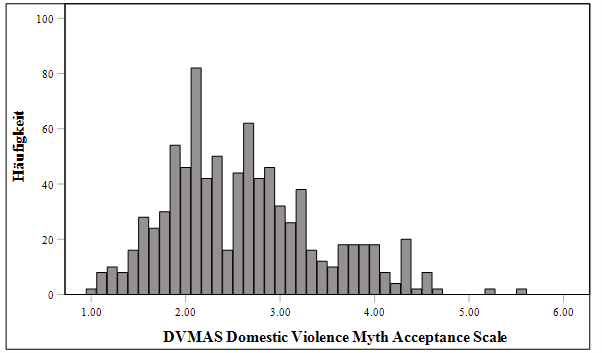
\includegraphics[width=0.8\linewidth]{Histogramm - DVMAS.png}
        \caption[Histogramm Altersverteilung]{Verteilung der Akzeptanz von Gewaltmythen.}
        \label{Histogramm DVMAS}
\end{figure}



\begin{figure}[htb!]
    \centering
        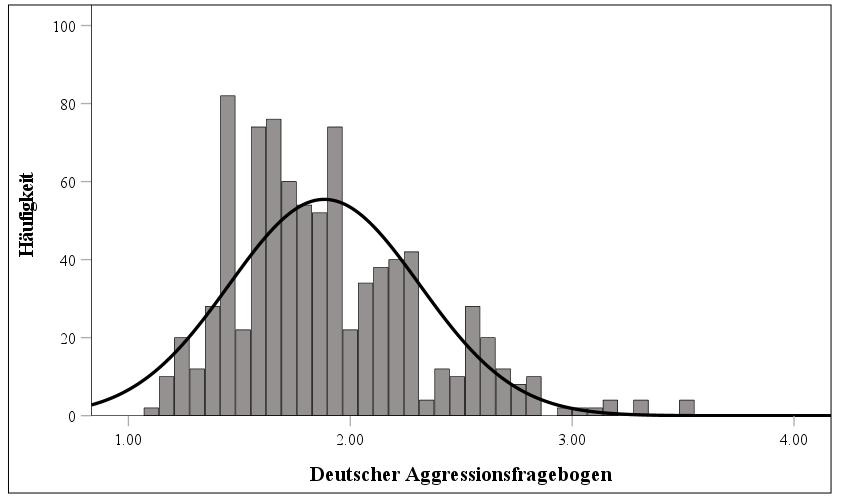
\includegraphics[width=0.8\linewidth]{Histogramm AggroFB.jpg}
        \caption[Histogramm Aggressionsfragebogen]{Verteilung der Angaben des Aggressionsfragebogens.}
        \label{Histogramm AggroFB}
\end{figure}


Beim Deutschen Aggressionsfragebogen wurde ein Mittelwert von $M$~=~1.88 ($SD$~=~0.43) und ein Median von $Mdn$~=~1.79 berechnet. Der geringste angegebene Wert betrug $Min$~=~1.10 und der höchste $Max$~=~3.52. Die Verteilung wies einen Schiefe von 0.94 und eine Kurtosis von 0.88 auf. Demzufolge ist die Verteilung rechstschiefe und hat eine breitgipflige Form, sowie eine Multimodalität mit den Modiwerten bei 1.59, 1.62, 2.52 und 2.55. Die Lageparameter weichen stark von den Normwerten ab. Diese sind wie folgt: $M$~=~2.66 ($SD$~=~0.88), Schiefe~=~3.81 und eine Kurtosis von -0.06. In Abbildung~\ref{Histogramm AggroFB} ist eine bildliche Darstellung der erhobenen Verteilung zu sehen. Die vorhandenen Ausreißer befinden sich alle unter der Ausscheidungsgrenze.
% Modus: 1.59, 1.62, 2.52, 2.55


\section{Manipulationscheck}    \label{sec_4.2}
Nachfolgend werden die Ergebnisse der vier Manipulationschecks in der folgenden Reihenfolge aufgeführt: Gewaltart, Geschlecht des Opfers, soziökonomischer Status der betroffenen Person und abschließend der Kulturelle Hintergrund.
Wie zuvor erklärt, musste der Datensatz verdoppelt werden, um eine berechnung mit den Daten gewährleisten zu können. Aus diesem Grund wird in diesem und den nachfolgenden Kapiteln von einer Stichprobengröße von $N_{neu}$~=~864 ausgegangen.

Bei der Überprüfung der Gewaltart gaben bei Vignetten sexualisierter Gewalt 354 Personen (91.70\%) an eine solche Gewaltart behandelt zu haben. Handelte es sich um eine psychische Gewaltart an, reichten nur 400 Personen (83.70\%) die richtige Antwort ein. Der durchgeführte Chi$^2$-Test viel mit einem Wert von 485.53 signifikant aus ($p<$.001). 

War die Nachfrage auf das Geschlecht des Opfers gerichtet gaben die 411 (96.70\%) bzw. 423 (96.40\%) Probanden an, es handelte sich um ein weibliches bzw. männliches Opfer. Auch dieser Chi$^2$-Test war mit einem Wert von 748.16 hoch signifikant ($p<$.001). 


Die Überprüfung des niedrigen soziökonomischen Status des Opfers wurde von 389 (80.2\%) bei dessen Gegebenheit richtig beanwortet. Bei der gegenteiligen Situation stieg die Rate der richtigen Antworten auf 342 (90.20\%). Mit einem Wert von 422.37 fiel dieser Chi$^2$-Test ebenfalls signifikant aus ($p<$.001). 

Die höchste Rate an Richtigkeit gab es bei dem Manipulationscheck des kulturellen Status. Hier gaben 422 (97.70\%) Personen bzw. 423 (97.90\%) die richtige Antwort. Auch dieser Chi$^2$-Test ist mit einem Wert von 789.68 signifikant ($p<$.001). 

\begin{table}[htb]
    \caption[Kreuztabelle Manipulationscheck]{\textit {Kreuztabelle der Manipulationschecks}} 
    \label{Kreuztabelle}
    \centering
    \begin{adjustbox}{width=\textwidth}
    \small
    \begin{tabular}{lrrrrrrrrr}
      \hline
        &   & psychisch & sexualisiert & weibliches Opfer & männliches Opfer & niedriger SES Opfer & hoher SES Opfer & arabisch & deutsch \\
      \hline
    Ja   & Anzahl  & 32      & \textbf{354}     & \textbf{411}      & 14      & \textbf{389}      & 96      & 10      & \textbf{422}      \\
         & Prozent & 8.30\%  & \textbf{91.70\%} & \textbf{96.70\%}  & 3.30\%  & \textbf{80.20\%}  & 19.8\%  & 2.30\%  & \textbf{97.70\%}  \\
    Nein & Anzahl  & \textbf{400}     & 78      & 16       & \textbf{423}     & 37       & \textbf{342}     & \textbf{423}     & 9        \\
         & Prozent & \textbf{83.70\%} & 16.30\% & 3.60\%   & \textbf{96.40\%} & 9.80\%   & \textbf{90.20\%} & \textbf{97.90\%} & 2.10\%   \\
       \hline
    \end{tabular}
    \end{adjustbox}
    
    \begin{tablenotes}
        \item \textit{Anmerkungen.} \( N_{neu} \)~=~864. SES = soziökonomischer Status. Prüffragen: (Gewaltart) Ging es um sexualisierte Gewalt? (Geschlecht) War das Opfer eine Frau? (SES) War die finanzielle Situation des Opfers schlechter als die finanzielle Situation des Täters? (Kultur) Hatten die Personen deutsche Namen?
      \end{tablenotes}
    \end{table}

    
In Tabelle ~\ref{Kreuztabelle} sind die Werte dieser Manipulationsprüfung nochmals zusammengefasst.


\section{Inferenzstatistische Ergebnisse}    \label{sec_4.3}
Ergebnisse der Hypothesentests


\subsection{Hypothese 1}    \label{subsec_4.3.1}
hier Vorraussetzungsergebnisse statistisch darlegen
% https://www.youtube.com/watch?v=ZPoYMfx0aIY (Vorraussetzung für Pearson)
metrische Skalen beider Variablen
keine Ausreißer
linearer Zusammenhang zwischen Variablen
Bivariate Normalverteilung -> zentralen Grenzwertsatz heranziehen/ mit Bootstraping arbeiten


\subsection{Hypothese 2}    \label{subsec_4.3.2}
hier Vorraussetzungsergebnisse statistisch darlegen
% https://www.youtube.com/watch?v=ZPoYMfx0aIY (Vorraussetzung für Pearson)
metrische Skalen beider Variablen
keine Ausreißer
linearer Zusammenhang zwischen Variablen
Bivariate Normalverteilung -> zentralen Grenzwertsatz heranziehen/ mit Bootstraping arbeiten


\subsection{Hypothese 3}    \label{subsec_4.3.3}
hier Vorraussetzungsergebnisse statistisch darlegen
%https://statistikguru.de/spss/moderation/voraussetzungen-14.html 
Linearität
Normalverteilung der Residuen (unwichtig, weil SP groß)
Homoskedastizität -> Schätzfehler über alle vorhergesagten y-Werte relativ gleich
Unabhängigkeit






Moderation: 14.31\% der Varianz des DVMAS werden durch das Modell erklärt.
Modell erklärt tatsächlich etwas, weil p kleiner .01 ist.
Grüne Linie: Geschlecht sorgt für höheren DVMAS-Wert bei gleichbleibender Aggression. Bei gleichbleibendem Aggressions-Score sorgt das Geschlecht für einen höheren DVMAS-Wert.

einen haupteffekt der signifikant ist der andere nicht, so wie die interaktion. Regressionsmodell mit 3 Prediktoren. eins hat n sig. Gewicht, der andere nicht.

Da die obere Grenze einen größeren Wert als 0 aufweist, ist die Interaktion nicht signifikant.

Eine Moderationsanalyse wurde durchgeführt, um zu bestimmen, ob die Interaktion zwischen Alter und Freizeit die Nutzung von sozialen Medien signifikant vorhersagt. Die Ergebnisse konnten keinen Moderationseffekt von Alter auf die Beziehung zwischen Freizeit auf Social Media-Nutzung finden, $\Delta R^{2}$ = 16.47\%, F(1, 96) = 18.93, p = .241, 95\% CI[-0.047, -0.015].


\section{Explorative Ergebnisse}    \label{sec_4.4}

